\documentclass[../main.tex]{subfiles}
\graphicspath{{\subfix{../Images/}}}
\begin{document}

\section{Sensors} \label{sensors}

% The Minion platform integrates multiple sensor modalities to support maritime perception research.
% This section details the specifications and characteristics of the visual cameras (Section~\ref{visual_cameras}) \ac{LiDAR} systems (Section~\ref{sensors_LiDAR}), and navigation sensors (Section~\ref{gps_ins}) used in this research.
% , thermal cameras (Section~\ref{thermal_cameras}), and navigation sensors (Section~\ref{gps_ins}) 

%%%%%%%%%%%%%%%%%%%%%%%%%%%%%%%%%%%%%%%%%%%%%%%%%%%%%%%%%%%%%%%%%%%%
\subsection{LiDAR} \label{sensors_LiDAR}

% The Minion platform features six \ac{LiDAR} units providing both omnidirectional environmental awareness and forward-facing high-density perception.
% The \ac{LiDAR} suite is comprised of three Velodyne VLP-16 pucks and three Livox Horizon units.

% Three Velodyne VLP-16 \ac{LiDAR} sensors are positioned at aft-center, with the other two placed at approximately one-third intervals around the vessel at forward-port and forward-starboard, providing complete 360-degree coverage for navigation as well as object detection and avoidance.
% An additional three Livox Horizon solid-state forward-scanning \ac{LiDAR} sensors provide high-density measurements within the forward direction of motion.
Three Velodyne VLP-16 \ac{LiDAR} sensors are installed around the vessel to provide omnidirectional situational awareness. 
One unit is mounted near the aft-center position, and the other two are positioned at approximately one-third intervals around the forward-port and forward-starboard quadrants. 
Together, these sensors deliver nearly continuous 360° coverage for navigation and obstacle avoidance.

Each VLP-16 employs 16 lasers arranged in a vertical array that scans 16 distinct points elevation over its 30-degree vertical \ac{FOV} continuously over the 360-degree azimuth, producing approximately 300,000 \ac{pps} in single-return mode. 
The units are installed with a downward declination of approximately 5 degrees from the plane of the \ac{USV} deck to minimize blind-spots near the vessel's waterline.
As a result, one-half to one-third of their scanning azimuth is well above the horizon or pointing directly into the vessel and is discarded, drastically reducing the number of points each unit can publish.

% Both of these units are capable of approximately 1.4 million measurements per second.
% For an equivalent 80-degree horizontal FOV, the Velodyne’s effective $317,700 \text{ pts/sec}$ represents $\approx 22 \%$ of the overlapping \ac{FOV} of the Livox unit’s output.
% % While each Velodyne VLP-16 unit is capable of producing 300k \ac{pps} compared to the Livox unit's 280k, their 360-degree scanning pattern means that only 
% The principal distinction between them lies in their underlying scanning architectures and sampling density, which directly influences perception fidelity.
% The Velodyne VLP-16 LiDAR scans 16 discrete points spanning a 30-degree vertical \ac{FOV} emanating from the azimuthal plane of the device in a 360-degree horizontal \ac{FOV}that repeats identically with each rotation. 
% The points generated span the 360
% % To minimize blind spots near the base of Minion, each of the Velodyne units is mounted at a 15-degree declination from the vessel's deck plane, resulting in 
% These rings are notF
% % For vessels moving at typical speeds (2-5 m/s), platform displacement between rotations remains small relative to object size, resulting in near-perfect overlap of consecutive scans.
% At typical vessel speeds between $2 \text{to} 5 m/s$, successive Velodyne rotations overlap almost perfectly, causing sparse sampling of small or distant targets.
% % This means that small to medium-sized objects may not even be detected when at large distances from the sensor, as illustrated in Figure \ref{fig:LiDAR_scan_compare}.
% Consequently, small or distant targets may be undersampled or entirely missed in sequential Velodyne frames (Figure \ref{fig:LiDAR_scan_compare}).

In contrast, the three Livox Horizon solid-state \ac{LiDAR} units concentrate their scanning pattern within an $81.7 \times 25.1$ degree \ac{FOV}, generating up to 280,000 \ac{pps}. 
Although the nominal point rates are comparable, the Livox pattern can return $100 \%$ of its concentrated \ac{FOV} data. 
This higher spatial sampling density enables detection and classification of objects that may be smaller or further from the sensor.
A direct comparison of the discrepancy between the Velodyne and Livox scan patterns and point density is provided in Figure \ref{fig:LiDAR_scan_compare}.
The top-right image shows the dense point cloud of the Livox devices.
The light tower in the foreground and the large dock structure in the background can be seen in the camera view (left) and are both well defined in the red point cloud.
Two small buoys are also distinctly visible between the two structures.
In comparison, the point cloud returned by the Velodyne devices is shown in the bottom-right. 
The general form of the light tower can be seen; however, there are very few points returned from the large dock structure in the background, and the round buoys are undetected.

% The forward-scanning Livox devices operate differently, tracing a non-repetitive pattern across the \ac{FOV}.
% Two orthogonal mirrors oscillate at slightly different frequencies to cause the laser beam to trace a path that progressively fills the \ac{FOV} without repetition as shown in Figure ~\ref{fig:livox_scan_pattern}.

\begin{figure}[htbp]
\centering
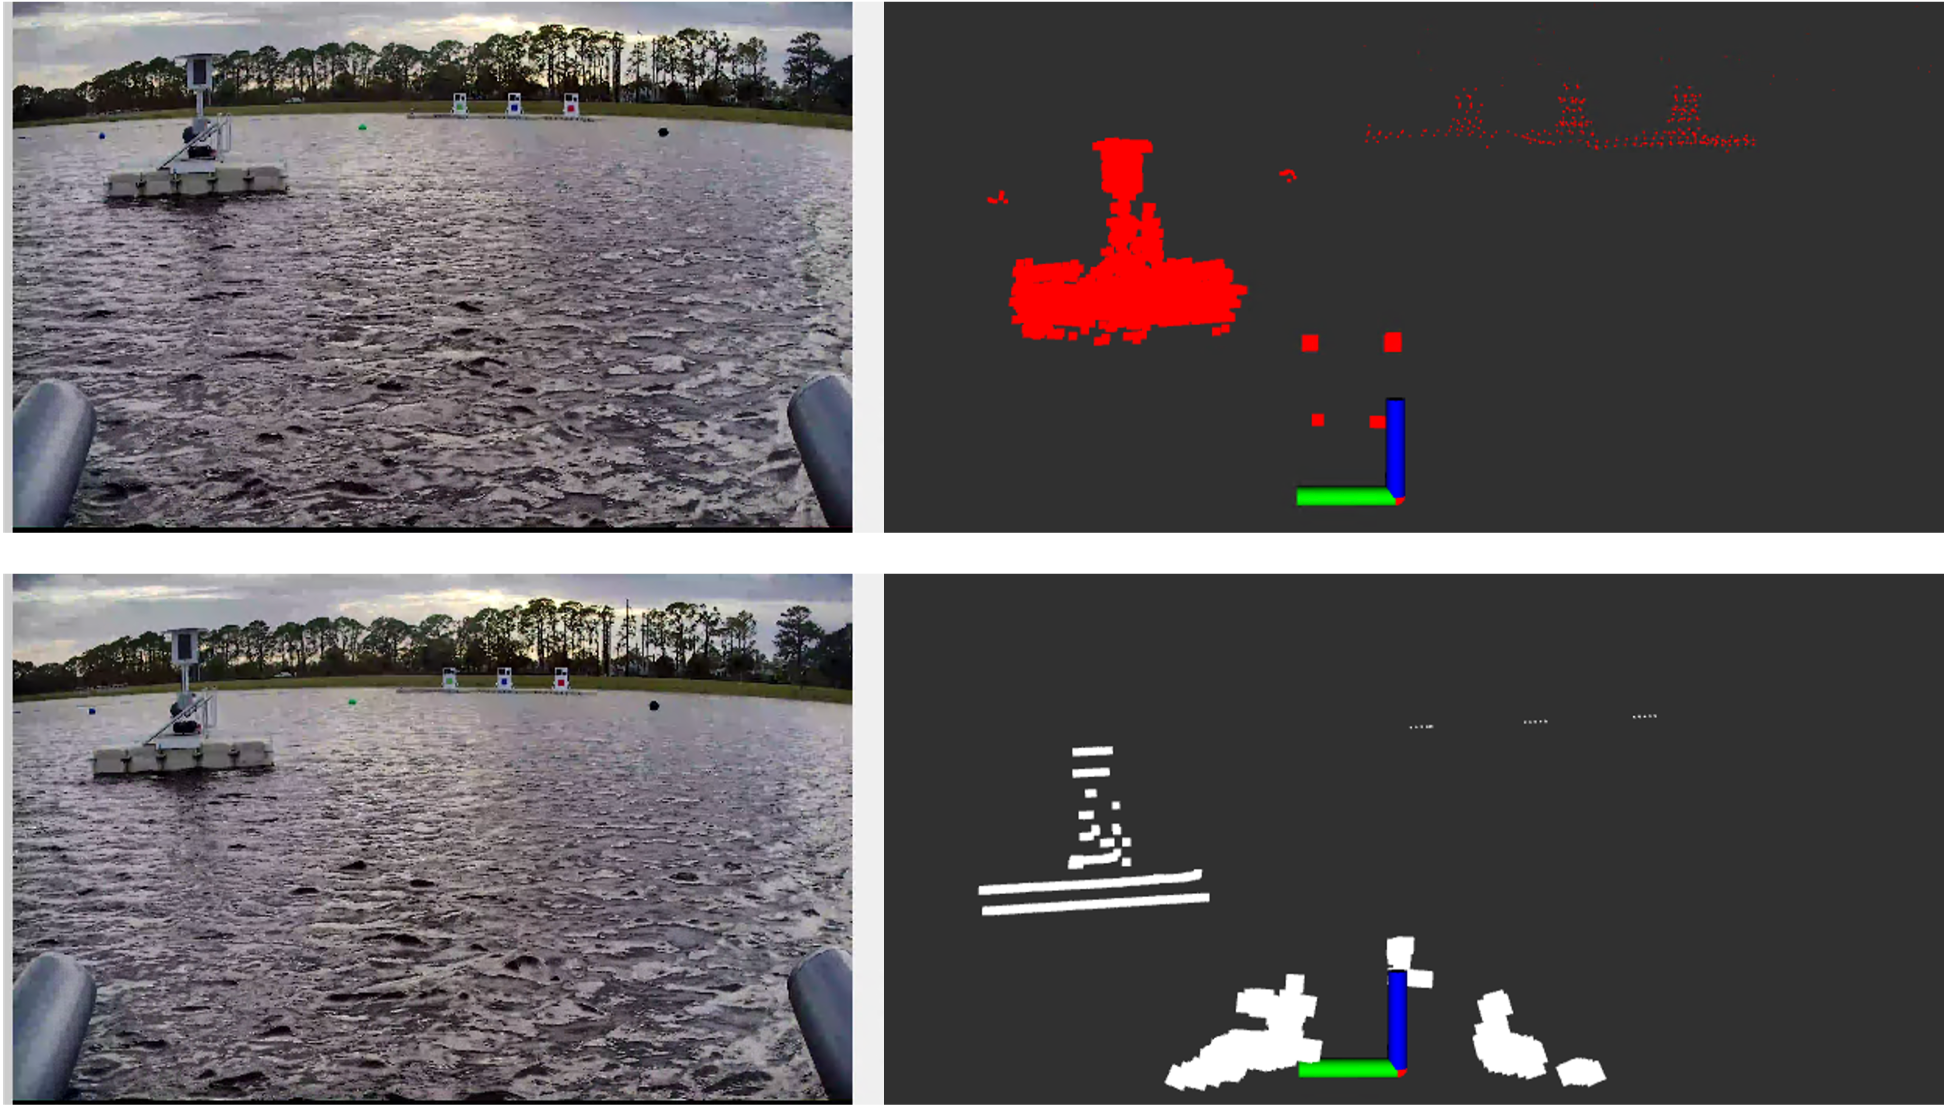
\includegraphics[width=0.8\textwidth]{Images/LiDAR_compare.png}
\caption{A comparison of LiDAR returns from the Livox units (top-right, red) and Velodyne units (bottom-right, white) to the respective HDR camera view (top-left and bottom-left). LiDAR points are viewed from third-person point of view in RVIZ. Green and Blue axes (top-right, top-bottom) represent the origin of the USV frame of reference.}
\label{fig:LiDAR_scan_compare}
\end{figure}

% The superior point density of the overlapping forward-scanning  LiDAR is critical for the real-time object detection method that is discussed in \textcolor{red}{Section \#}.
% The overlapping forward-scanning LiDAR provides the spatial density required for the real-time object-detection framework described in Section \ref{gbcache}.
% For this reason, the research presented in this work exclusively utilizes LiDAR data from the Livox Horizon sensors.

Consequently, the research presented in this work relies exclusively on LiDAR data from the forward-scanning Livox Horizon sensors, whose concentrated and non-repetitive coverage provides the spatial resolution required for the real-time object-detection framework described in Section \ref{gbcache}.
        %%%%%%%%%%%%%%%%%%%%%%%%%%%%%%%%%%%%%%%%%%%%%%%%%%%%%%%%%%%%
\subsubsection{Livox Horizon} \label{sensors_livox}

% Each Livox Horizon employs two orthogonal mirrors operating at different frequencies to trace a complex Lissajous-like path that progressively fills the $81.7 \times 25.1$-degree (horizontal × vertical) \ac{FOV}, as illustrated in Figure~\ref{fig:livox_scan_pattern}. 
% The three Livox units are mounted with 40 degrees of horizontal separation, overlapping each other \ac{FOV} by $\approx 50\%$, making the system robust to failure of any single unit, as well as effectively doubling the rate of sampled points and distributing them more evenly across the center device's \ac{FOV}. 
Each Livox Horizon uses dual orthogonal mirrors oscillating at slightly different frequencies to generate a non-repetitive Lissajous-like scan pattern over its $81.7 \times 25.1$ degree \ac{FOV}. 
Overlapping these sensors by roughly $50 \%$ effectively doubles the point density along the center-line path under nominal operation, and maintains coverage under single-unit failure.
Table~\ref{table:livox_horizon_specs} presents detailed hardware specifications for the Livox Horizon.

% The rosette scan pattern is provided in \ref{fig:livox_scan_pattern}, and table \ref{table:livox_horizon_specs} presents the Livox Horizon specifications.

\begin{figure}[htbp]
\centering
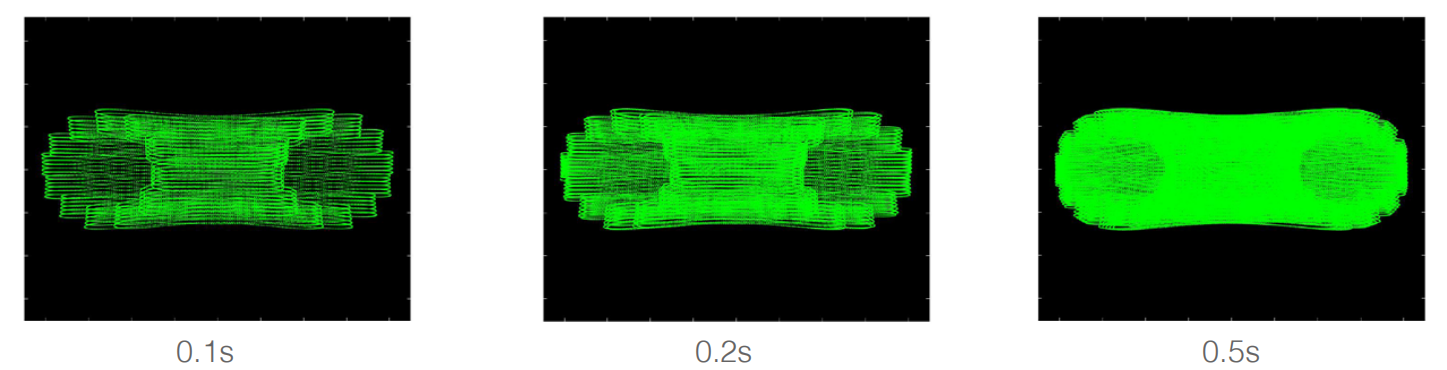
\includegraphics[width=0.8\textwidth]{Images/Livox_1.png}
\caption{Accumulation of points with the Livox Horizon's non-repetitive scan pattern, from 0.1 to 0.5 seconds  \cite{livox_manual}.}
\label{fig:livox_scan_pattern}
\end{figure}

Each device is capable of returning up to $4.8 \times 10^5$ \ac{pps} in dual return mode, with each return consisting of position coordinates (x, y, z), target reflectivity, and timestamp.
This operational mode returns two data points for each laser emission and is useful for situations where the sensor scans semi-permeable objects such as windows, thick tree canopies, or water.
% Instead, each device is operated in single-return mode for two reasons.
% The first is a consideration of available network bandwidth.
Each sensor operates in single-return mode, primarily to reduce network load.
A conservative estimate of 16 bytes per point results in $\approx 23 \text{ Mbps}$ which would quickly overwhelm the \ac{USV}'s network.
% Luckily, the 905 nm near-infrared wavelength of the emitted laser experiences strong absorption by water. 
However, The $905 nm$ near-infrared emission is strongly absorbed by water, effectively suppressing subsurface returns.
This means that only points which are reflected by the water surface are returned with an intensity greater than zero, making it straight forward to filter out points in the ground plane.

\begin{table}[htpb]
\centering
\begin{tabular}{ll}
\hline
\multicolumn{2}{c}{Livox Horizon}\\
\hline
% \textbf{Parameter} & \textbf{Value} \\
\hline
Model & Livox Horizon \\
Horizontal Field of View & 81.7 degree \\
Vertical Field of View & 25.1 degree \\
Range & 260 m @ 80\% reflectivity \\
Point Rate (Single Return) & 240,000 pts/sec \\
Point Rate (Dual Return) & 480,000 pts/sec \\
Range Precision & ±2 cm \\
Wavelength & 905 nm \\
Scan Pattern & Non-repetitive rosette \\
Interface & Ethernet \\
Operating Frequency & 100 Hz \\
\hline
\end{tabular}
\caption{LiDAR Specifications}
\label{table:livox_horizon_specs}
\end{table}

%%%%%%%%%%%%%%%%%%%%%%%%%%%%%%%%%%%%%%%%%%%%%%%%%%%%%%%%%%%%%%%%%%%%
\subsection{Visible Spectrum Cameras} \label{visual_cameras}

% \textcolor{red}{Expand this entire discussion}
% The visible spectrum camera suite on the Minion platform is designed to balance two factors that are particularly important for maritime perception: imaging resolution and dynamic range.

For computer vision and perception tasks, system performance is directly influenced by the quality of the visual input.
The fidelity of an image is determined by a camera's hardware and integrated software; therefore, camera selection is a critical design consideration in any vision-based system. 
Sensor size and lens characteristics determine the spatial detail captured, while shutter speed, exposure, and onboard processing influence brightness, contrast, and color balance. 
The visible-spectrum cameras housed within the camera enclosure were selected to balance image resolution and dynamic range, two essential factors for reliable maritime perception.
A brief discussion of both of these metrics is presented here to justify utilizing data acquired from the \ac{HDR} camera for this research.

\subsubsection{Image Resolution}
Camera resolution determines the ability to resolve small targets at a distance.
% , and appropriate imaging sensors and lenses can be selected by determining the maximum distance and minimum size at which objects need to be resolved.
% Camera resolution dictates the minimum discernible target size at range; lens and sensor parameters are therefore chosen to meet specified detection distances.
% Camera resolution governs the minimum resolvable target size; lens and sensor parameters are thus selected to ensure detection at required ranges.
To ensure adequate perception across the operational envelope, cameras must resolve objects to a required minimum resolution when the object is at the maximum detection range.
% The resolution of an object in the image frame can be determined if the object's width $\mathit{l}$ and distance from the camera $d$ are knownwith
The relationship between an object's physical width $\mathit{w}_{obj}$ and pixel width within an image $\mathit{w}_{\text{px}}$ is given by
% Provided a maximum detection range $d$ and the width of the smallest object to be detected $W$, the camera's focal length and resolution requirements can be determined by assuming a pinhole-camera model \cite{matlab_calibration}, can be derived as:
% we can determine the necessary optical focal length and resolution for the sensor.
% For an object of physical width $W$ at distance $d$, its width in the image frame $w_{\text{px}}$ is approximated by

\begin{equation}
\mathit{w}_{\text{px}} = f \; \frac{N_x}{S_w}\frac{\mathit{w}_{obj}}{d}
\end{equation}

% where $\mathit{l}_{\text{px}}$ is the pixel width of an object in the image frame, 
where $f$ is the \ac{EFL} of the camera and lens, $N_x$ is the horizontal image resolution in pixels, and $S_w$ is the width of the image sensor.
% This equation is used for sensor selection by determining the minimum resolution required for the smallest object to be detected at the maximum detection range.
This equation can be used to determine camera requirements if the true size of the imaged objects is known, or to determine a reasonable expectation of object resolution if the camera values are known.
This relationship is also critical for determining the distortion present in each camera/lens system, detailed further in section~\ref{spatial_calibration}.

Defining the requirement for the minimum resolution of an object in the image frame requires an understanding of the object detection method used with visual cameras, as well as the objects being detected. both of which will be discussed in greater detail in sections ~\ref{sec:sensor_data_dataset} and ~\ref{yolo}, respectively.
% For now, it is sufficient to know that the smallest object we wish to detect is $0.3683$ meters wide at a distance of 60 meters.
% , and that we have optical and digital resolution requirements to consider.
This image detection architecture is discussed in section ~\ref{yolo}.
For camera selection, it is sufficient to know that this method scales down each input image to a resolution of $640 \times 640$ pixels for processing efficiency.
This should be considered when defining the minimum pixel density of a camera's sensor, as it alters our prior equation slightly.

\begin{equation}
\mathit{w}'_{\text{px}} = f \; \frac{640 \text{px}}{S_w}\frac{\mathit{w}_{obj}}{d}
\end{equation}
% This means that an image captured at $4000 \times 3000$ pixels is reduced to $650 \times 487$ pixels, which is $16.25\%$ of its original size.
% As an example, if the text on waterway signage 60 meters away is legible at a resolution of 100 pixels wide in a 1,000 $\times$ 1,000 pixel image, it would need a resolution of 162 pixels to meet the additional requirements imposed by the image detection algorithm.
Each camera within the enclosure was selected using these metrics, and object information based on the obstacles commonly associated with the RobotX Maritime Challenge. %, in addition to other contemporaneous research \cite{thompson2023} \textcolor{red}{(check scholarly commons)}.

% \textcolor{red}{add back: ?}
Given that the smallest object we wish to detect is $0.3683$ meters wide at a distance of 60 meters.
The two visual spectrum camera models within the camera enclosure have a similar focal length, and resolutions of $4000 \times 3000$ px and $2880 \times 1860$ px. Examining the camera with the smaller horizontal resolution of 1880 px (which has a sensor width of $S_{w} = 8.64$ mm), we obtain the width of our object in the image frame as
% meet this requirement; the object detection method used will impose a secondary constraint.
\begin{equation*}
\begin{split}
    \mathit{w}_{\text{px}} & = 8\;\text{mm} \cdot \frac{2880\;\text{px}}{8.64\;\text{mm}} \cdot \frac{0.3683\;\text{m}}{60\;\text{m}}\\
     & = 16.36 \approx 16 \;\text{px}
\end{split}
\end{equation*}

With the additional scaling required by the visual object detection method, the minimum width of our object becomes 
\begin{equation*}
\begin{split}
    \mathit{w}'_{\text{px}} & = 16\;\text{px} \cdot \frac{640\;\text{px}}{2880\;\text{px}} \\
     & = 3.\overline{55} \approx 3 \;\text{px}
\end{split}
\end{equation*}

Figure \ref{fig:A2_multi_res} shows our smallest object, Polyform A2 round buoy, at a selection of resolutions, and is still recognizable at a resolution of 16 pixels wide. %, and becomes less defined at lower resolutions. 
This operation is repeated to predict the width of the object in the image frame at a range of distances up to our maximum of 60 meters, and the results are provided in Table \ref{table:buoy_res}.
From this information, the buoy will be easily recognizable at any range by visual inspection, but will become much less defined when the image is scaled down for the visual object detection method.
As we will discuss in section \ref{yolo}, this method may struggle to detect this size buoy at distances greater than 20 meters.

\begin{table}[htpb]
\centering
\begin{tabular}{c|c|c}
\hline
\multicolumn{3}{c}{Polyform A2 Buoy Resolution at Range}\\
\hline
% \textbf{Parameter} & \textbf{Value} \\
\hline
Object Distance & Image Frame Width & With Detection \\
\hline
10 m & 98 px & 21 px \\
20 m & 49 px & 10 px \\
30 m & 32 px & 7 px \\
40 m & 24 px & 5 px \\
50 m & 19 px & 4 px \\
60 m & 16 px & 3 px \\
\hline
\end{tabular}
\caption{The predicted resolution of a $\mathit{l} = 0.3683$ meter wide object within the Loepard Imaging HDR camera's image frame at multiple distances.}
\label{table:buoy_res}
\end{table}

\begin{figure}[htbp]
\centering
\begin{subfigure}[t]{0.245\textwidth}
    \centering
    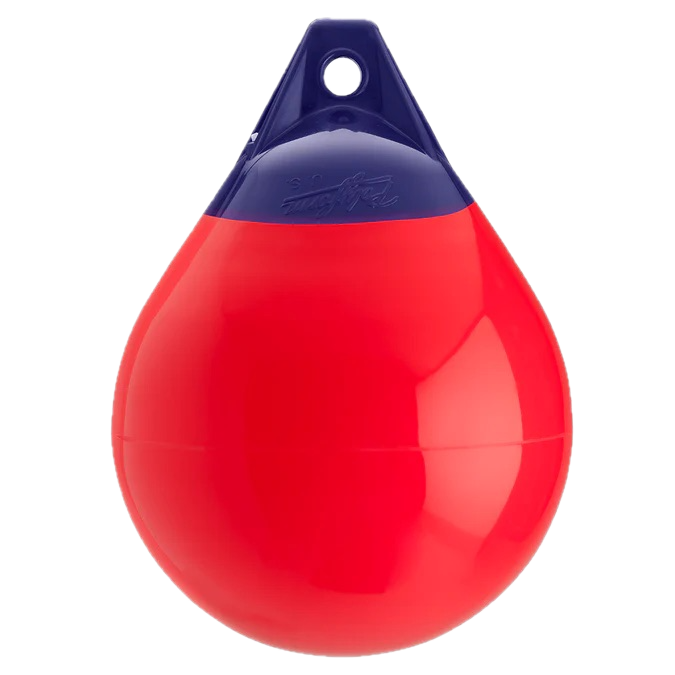
\includegraphics[width=\textwidth]{Images/A2.png}
    \caption{\raggedright{Polyform A2 Buoy}}
    \label{fig:A2}
\end{subfigure}
\hfill
\begin{subfigure}[t]{0.245\textwidth}
    \centering
    
\includegraphics[width=\textwidth]{Images/A2_16px.png}
    \caption{
    16 pixel width,\\  
    % $\approx$ 60 m with HDR
    }
    \label{fig:A2_16px}
\end{subfigure}
\hfill
\begin{subfigure}[t]{0.245\textwidth}
    \centering
    
\includegraphics[width=\textwidth]{Images/A2_6px.png}
    \caption{
    6 pixel width,\\  
    % $\approx$ 40 m with HDR \\ 
    % \& object detection.
    }
    \label{fig:A2_6px}
\end{subfigure}
\hfill
\begin{subfigure}[t]{0.245\textwidth}
    \centering
    
\includegraphics[width=\textwidth]{Images/A2_3px.png}
    \caption{
    3 pixel width,\\  
    % $\approx$ 60 m with HDR \\ 
    % \& object detection.
    }
    \label{fig:A2_3px}
\end{subfigure}
\caption{Polyform A2 Buoy (a), visualized at 16 pixels (b), 6 pixels (c), and 3 pixels wide (d).}
\label{fig:A2_multi_res}
\end{figure}




% The dynamic range of an imaging sensor refers to the range of signal intensities it can detect, and can be as critical as image resolution when selecting camera sensors.
\subsubsection{Dynamic Range}
Dynamic range describes the ratio between the brightest and darkest signal levels a camera sensor can record.
Light levels that exceed the camera sensor's range cause the image to appear white or "blown-out", while light levels that are too low will appear darker, with detail being indistinguishable from noise.
% Dynamic range—the span of detectable signal intensities—is equally critical to sensor selection as spatial resolution.
\acp{USV} and \acp{AGS} routinely operate in environments where bright sky reflections and deep shadows are common, often within the same scene.
Therefore, selecting a camera with insufficient dynamic range may lead to washed-out highlights or lost detail in shadows.

Dynamic range, expressed in dB, is given by
\begin{equation}
 \text{Dynamic Range (dB)} = 20 \log{\left( \frac{N_{sat}}{N_{noise}}\right) }
\end{equation}
where $N_{sat}/N_{noise}$ is the ratio of the saturation to the minimum signal a camera sensor can detect above background noise.
% Higher dynamic range can be achieved through software by combining sequential multi-exposure images, or through a digital overlap \ac{HDR} (DOL-HDR) architecture with in-pixel dual conversion gain.
% Sequential multi-exposure \ac{HDR}, which stacks separate frames and is prone to ghosting or blurring, therefore 
% DOL-\ac{HDR} is preferred when precise synchronization of the imagery is required, such as sensor fusion.
% Because maritime environments routinely present both bright sky reflections and deep shadows in the same scene, dynamic range is as critical as resolution when selecting cameras for perception tasks. 
High-dynamic-range (HDR) imaging can be achieved in two primary ways. 
The first is sequential multi-exposure \ac{HDR}, in which multiple frames captured at different exposure settings are combined to extend the tonal range \cite{Reinhard2010}. An example is provided in Figure \ref{fig:hdr_example}.



While effective for static scenes, this approach introduces motion-related artifacts such as ghosting and motion-blur as the relative velocity increases between the sensor and objects within the frame.
The second method uses an in-sensor technique called dual-conversion gain (DCG) that combines multiple light exposure levels within a single frame of exposure. 
% \textcolor{red}{Coyle: It isn't short and long exposure, but changing the size of the exposure pixel to capture more/less light from my understanding. This is why it doesn't motion blur} By capturing short and long exposure data within a single frame, this method avoids the distortion of multi-exposure \ac{HDR}.
The two visible sensing technologies considered for this research are described below.

\begin{figure}[htbp]
    \centering
    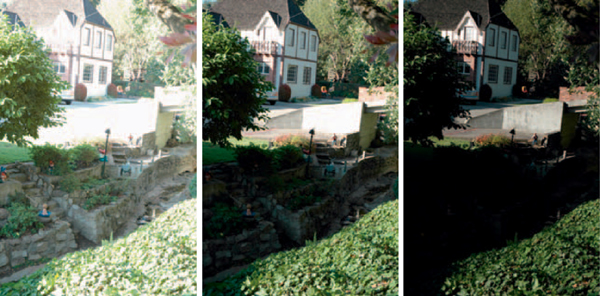
\includegraphics[width=0.65\linewidth]{Images/hdr_example.png}
    \caption{An example of multi-exposure HDR frame-stacking \cite{Reinhard2010}.}
    \label{fig:hdr_example}
\end{figure}
%%%%%%%%%%%%%%%%%%%%%%%%%%%%%%%%%%%%%%%%%%%%%%%%%%%%%%%%%%%%%%%%%%%%
\subsubsection{FLIR Blackfly S 4K Cameras} \label{sensors_FLIR}

% Three FLIR Blackfly S 4K visible-light cameras, arranged to provide a combined 165 degrees of forward-facing coverage through overlapping 65-degree lenses.  
Three FLIR Blackfly S 4K cameras are aligned to the port, center, and starboard sight-lines described in section \ref{perception_geometry} to provide a combined 165-degree horizontal \ac{FOV}.
In addition to redundancy, this configuration avoids additional spherical distortion within the image that would be required to cover the same \ac{FOV} with fewer cameras.
% Each camera is paired with a Theia TL410P zoom lens with an \ac{EFL} of \textcolor{red}{???} and an image resolution of $4096 \times 4096$, ensuring that objects remain adequately resolved across the vessel's perception envelope.  
Each FLIR Blackfly has a resolution of 4096 $\times$ 4096 pixel resolution and is paired with a Theia TL410P zoom lens at a fixed \ac{EFL} $\approx$ 8 mm.
% This sensor dimension and \ac{EFL} exceeds the pixel density required to ensure object resolution across the operational envelope.


\begin{table}[htbp]
\centering
\begin{tabular}{ll}
\hline
\multicolumn{2}{c}{FLIR 4K SDR Camera}\\
% HDR & Camera\\
\hline
% \textbf{Parameter} & \textbf{Value} \\
\hline
\multicolumn{2}{c}{Camera Sensor}\\
\hline
FLIR & Blackfly S 120S4C \\
% Image Sensor & Sony IMX490 \\
% Pixel Size & $3.0 \times 3.0 \mu m$ \\
Horizontal Resolution & 4000 pixels \\
Vertical Resolution & 3000 pixels \\
Aspect Ratio & 1.33:1 \\
Maximum Frame Rate & 31 fps \\
Dynamic Range & 69.4 dB \\
\multicolumn{2}{c}{Camera Lens}\\
\hline
Theia & TL410P\\
% Aperture F/\# & $2.0$ \\
Horizontal \Ac{FOV} & 65-degrees\\
Lens \Ac{EFL} & approx. 8 mm\\
% Vertical Field of View & 37 degrees \\
\hline
\end{tabular}
\caption{FLIR 4K SDR Camera Specifications}
\label{table:SDR_camera_specs}
\end{table}

The Blackfly S sensor captures video at 31 \ac{fps} and achieves a dynamic range of 69.4 dB, which is within the \ac{SDR}.
% This corresponds to a span of a few thousand-to-one between the darkest detectable signal and the brightest non-saturating signal.  
% The cameras capture 31 \ac{FPS} at a resolution of 4096 $\times$ 2160 pixels.
% \textcolor{red}{Add discussion of pixel density sensor selection in the context of the requirement to resolve specific objects at a minimum resolution at a maximum specific distance. This will require equations.}

%%%%%%%%%%%%%%%%%%%%%%%%%%%%%%%%%%%%%%%%%%%%%%%%%%%%%%%%%%%%%%%%%%%%
\subsubsection{Leopard Imaging HDR Camera} \label{sensors_HDR}

% A Leopard Imaging LI-USB30-IMX490-GW5400-GMSL2-065H camera, based on Sony’s IMX490 automotive-grade \ac{HDR} sensor, provides 65-degree of forward \ac{FOV}.  
The Leopard Imaging camera provides a 65-degree forward \ac{FOV} using Sony’s automotive-grade IMX490 sensor with 120 dB of dynamic range.
The \ac{HDR} is achieved via Sony’s \ac{DOL-HDR} architecture, which combines large and small photodiodes within each pixel on the sensor.
Each size of sub-pixels experience a different photon flux during each frame of exposure, and each output is read at both high and low conversion gains.
This method yields 4 measurements of light intensity within each captured frame, eliminating motion artifacts and enabling precise temporal alignment for sensor fusion.
Table \ref{table:hdr_camera_specs} provides detailed specifications for the HDR camera, which delivers a resolution of $2880 \times 1860$ pixels at 25 frames per second with a dynamic range of 120~dB
% Sony’s \ac{DOL-HDR} architecture exposes both sub-pixels (SP1 and SP2) simultaneously but reads them sequentially at different conversion gains to capture multiple brightness levels within a single frame.
% It utilizes two sizes of sensing pixels, one large and one small, which receive different flux of of photons per exposure,  within a single frame period. \textcolor{red}{Coyle: use same terminology as where you described this earlier.}
.%, extending the span of detectable light intensity to nearly one million-to-one.  

% The IMX490 accomplishes this \ac{HDR} using a digital overlap \ac{HDR} (DOL-HDR) architecture with in-pixel dual conversion gain.  

% This method captures multiple effective exposures within a single frame period, producing simultaneous multi-gain readouts from the same scene.  
% This architecture produces simultaneous multi-gain readouts without sequential stacking, 

\begin{table}[htpb]
\centering
\begin{tabular}{ll}
\hline
\multicolumn{2}{c}{Leopard Imaging HDR Camera}\\
% HDR & Camera\\
\hline
% \textbf{Parameter} & \textbf{Value} \\
\hline
% Make & Leopard Imaging \\
Leopard Imaging & LI-IMX490-GW5400-GMSL2-065H \\
Image Sensor & Sony IMX490 \\
Pixel Size & 3.0 $\times$ 3.0 $\mu$m \\
Horizontal Resolution & 2880 pixels \\
Vertical Resolution & 1860 pixels \\
Aspect Ratio & 1.55:1 \\
Maximum Frame Rate & 25 fps \\
Dynamic Range & 120 dB \\
Aperture F/\# & $2.0$ \\
Horizontal \Ac{FOV} & 65-degrees \\ %(H), 37-degrees (V) \\
% Vertical Field of View & 37 degrees \\
Lens \Ac{EFL} & 7.9 mm\\
\hline
\end{tabular}
\caption{Leopard Imaging HDR Camera Specifications}
\label{table:hdr_camera_specs}
\end{table}


%%%%%%%%%%%%%%%%%%%%%%%%%%%%%%%%%%%%%%%%%%%%%%%%%%%%%%%%%%%%%%%%%%%%
\subsubsection{Camera Selection} \label{camera_selection}

The combination of image resolution and \ac{EFL} of both cameras exceeds the pixel density required to ensure object resolution across the operational envelope.
\textcolor{red}{Coyle: which you never told me}
FLIR Blackfly S 4K cameras exceed the resolution requirements, but their limited dynamic range of 69.4~dB makes them prone to over-exposure and reduced contrast under extreme lighting conditions. 
% They support an effective dynamic range of 69.4~dB, which corresponds to a span of just a few thousand-to-one between the darkest detectable signal and the brightest non-saturating signal. 
% As a result, the cameras are prone to over-exposure in high-brightness maritime conditions, particularly when imaging reflective water surfaces or bright sky backgrounds, leading to loss of highlight detail and reduced contrast. 

\begin{figure}[htbp]
\centering
\makebox[\textwidth][c]{%
    \begin{subfigure}[t]{0.35\textwidth}
        \centering
        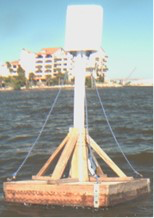
\includegraphics[width=\textwidth]{Images/SDR_bright.png}
        \caption{SDR visual camera (5 MP)}
        \label{fig:SDR_bright}
    \end{subfigure}
    \hspace{2em} % horizontal spacing between them
    \begin{subfigure}[t]{0.378\textwidth}
        \centering
        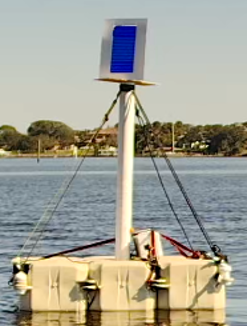
\includegraphics[width=\textwidth]{Images/HDR_bright.png}
        \caption{HDR visual camera (5 MP)}
        \label{fig:HDR_bright}
    \end{subfigure}%
}
\caption{\textcolor{red}{place-holder image – A visual comparison of the \ac{SDR} FLIR 4k camera (left) and the \ac{HDR} Leopard Imaging camera (right) in low-light conditions.}}
\label{fig:HDR_compare}
\end{figure}

In contrast, the Leopard Imaging \ac{HDR} camera offers slightly lower image resolution at a comparable effective focal length but provides substantially greater dynamic range.
% enabling detail preservation across bright and shaded regions within the same frame.  
This wider dynamic range enables more consistent color fidelity and image contrast under suboptimal lighting conditions, as illustrated in Figure~\ref{fig:HDR_compare}.

% Many tasks in the 2024 Maritime RobotX Challenge required \acp{USV} to accurately distinguish object colors as part of their operational decision-making.
This capability motivated the selection of the \ac{HDR} camera as Minion's primary visual camera sensor for the 2024 Maritime RobotX Challenge, which included several tasks that required \acp{USV} to accurately identify object colors in order to make operational decisions.
\textcolor{blue}{Check these results again}\textcolor{blue}{A comparative study by Liebergall et al.~\cite{liebergall} further supported this decision, as preliminary results indicated improved object detection results with data from the \ac{HDR} over the FLIR \ac{SDR} camera.}
Because the data collected during that competition formed the foundation of this dissertation, the Leopard Imaging \ac{HDR} camera, the primary visual spectrum sensor, was selected for all research presented in this paper.

% For these reasons, the \ac{HDR} camera was designated as the primary forward-facing visual spectrum sensor for the \ac{LiDAR}-camera fusion research presented in this paper.  




%%%%%%%%%%%%%%%%%%%%%%%%%%%%%%%%%%%%%%%%%%%%%%%%%%%%%%%%%%%%%%%%%%%%
%%%%%%%%%%%%%%%%%%%%%%%%%%%%%%%%%%%%%%%%%%%%%%%%%%%%%%%%%%%%%%%%%%%%

\subsection{PinPoint GPS/INS} \label{sensors_GPS}

% The Minion platform features a PinPoint \ac{GPS}/\ac{INS} equipped with dual-antennae for orientation and differential corrections for millimeter precision geolocation.
% The sensor performs two critical functions for the \ac{USV}: tracking vessel position and orientation, and precise global time for sensor synchronization.
% The \ac{GPS} receiver functions as the master clock for the entire synchronization hierarchy described in ~\ref{time_sync}, while the integrated \ac{IMU} enables high-rate pose updates between \ac{GPS} fixes.

The Minion \ac{USV} employs a Torc Robotics Pinpoint \ac{GPS}/\ac{INS} unit for both global positioning and inertial navigation capabilities.
This device integrates a differential-corrected \ac{GPS} receiver with a multi-axis \ac{IMU} and dual antenna, providing precise position, velocity, and orientation data for the autonomous platform.
The \ac{GPS} receiver is configured to operate at an update rate of five Hz, while the integrated \ac{IMU} provides high-frequency inertial measurements at 105.4 Hz.
The Pinpoint unit delivers timing accuracy on the order of 10-100 nanoseconds for \ac{GPS}-disciplined time signals, which is a critical function for multi-sensor synchronization discussed in Section~\ref{time_sync}.


%%%%%%%%%%%%%%%%%%%%%%%%%%%%%%%%%%%%%%%%%%%%%%%%%%%%%%%%%%%%%%%%%%%%
%%%%%%%%%%%%%%%%%%%%%%%%%%%%%%%%%%%%%%%%%%%%%%%%%%%%%%%%%%%%%%%%%%%%

\end{document}
